% !TeX root = ../../main.tex


\section{井筒内砂砾运移及分布规律研究}

\subsection{砂砾在环空中的运移及分布}\label{sec:sand_sendiment_circular_section}

洗井作业中，冲砂工具和管柱的砂堵问题直接影响作业安全与效率。砂堵的本质是砂砾在工具与井筒环空内的异常堆积，不仅会导致工具功能失效、卡钻、冲砂液循环中断，还会导致非计划停工、设备维修成本攀升。通过仿真研究井筒内工具与井筒环空砂砾运移规律，可以预测砂砾在井筒环空内的运移速度以及沉积规律，为冲砂作业提供理论指导。现场提供的砂砾样本（见图\ref{fig:sand_sample}）及其粒度分级统计数据（参见表\ref{tab:real_sand_parameter}），后文的模拟都以此为依据。

\begin{figure}[htbp]
	\centering
	\includegraphics[width=0.5\textwidth]{figure/sand-sample.jpg}
	\caption{井筒出砂样本}
	\label{fig:sand_sample}
\end{figure}

\begin{table}[H]
	\centering
	\caption{砂砾粒度分级统计}
	\label{tab:real_sand_parameter}
	\begin{tabularx}{.9\textwidth}{CCC}
		\toprule
		分类 & 粒级区间/\(\mu\)m & 含量/\% \\
		\midrule
		砾石 & \(\geq 2000\) & $0.00$ \\
		巨砂 & $2000.00$--$1000.00$ & $0.00$ \\
		粗砂 & $1000.00$--$500.00$ & $1.03$ \\
		中砂 & $500.00$--$250.00$ & $35.29$ \\
		细砂 & $250.00$--$125.00$ & $47.15$ \\
		极细砂 & $125.00$--$62.50$ & $13.99$ \\
		粗粉砂 & $62.50$--$31.25$ & $1.92$ \\
		细粉砂 & $31.25$--$3.90$ & $0.61$ \\
		粘土 & \(\leq 3.90\) & $0.00$ \\
		\bottomrule
	\end{tabularx}
\end{table}


% \subsubsection{幂律流体}

% 钻井液属于非牛顿流体，其本构方程符合幂律流体，流变参数
% \begin{equation}
% 	\tau=K\dot{\gamma}^{n}
% \end{equation}
% 其中，\(K\) 为钻具内钻井液稠度系数，\(n\) 为钻井液流变指数。依据相关文献，\(K=2.38\)，\(n=0.80\)。


实际油气井筒长度较大且井眼轨迹变化缓慢，模拟条件下，难以对其进行整体等比例复现。因此，本模拟采用长度较短、曲率较大的局部弯曲管段模型，重点研究井斜变化及弯曲段内砂砾的运移规律。虽然实验模型的长度和曲率与实际井筒存在差异，但砂砾的沉降、悬浮和随流迁移等局部运动行为主要受环空几何尺寸、流体流动参数、颗粒性质及重力作用控制，其特征长度尺度远小于实际井筒长度。实验模型按照实际井筒的环空尺寸和洗井工况设置边界条件，使模型能够反映颗粒在局部环空内的主要受力和运动状态；同时，较大的曲率可在有限实验空间内集中体现井斜变化对颗粒运移的影响，便于观察和比较不同井斜条件下的运移特性。因此，该模型虽不能完全复现实际井筒的整体尺度和轨迹，但能够有效反映局部弯曲环空内砂砾运移的主要机制及变化规律，可用于分析洗井液流动参数和井斜角对砂砾运移特性的影响。%交叉验证

本文建立的全井筒模型三维结构如图\ref{fig:annular_3d_model}所示，水平井模型长 \(L = 1.5\) m，取曲率半径 \(1\) m、总弯曲角为 \(90^{\circ}\) 的水平+圆弧弯管模型模拟一个完整的水平井。流域几何由井壁、光滑钻杆表面及进出口围成，采用多面体单元对所建模型进行网格划分。根据实际工况，在洗井过程中，井筒环空中的砂砾会受到洗井液冲击而发生运动，环空内部流动环境复杂，属于典型的液--固两相湍流流场，因此，本节采用欧拉两相流模型对环空砂砾运移进行数值模拟，并将环空流场视为稳定的不可压缩湍流流场。为了简化两相流，本节假设砂砾是尺寸均匀的球形。根据正循环洗井工况进行边界条件的设置，入口（趾端）定义为洗井液和砂砾颗粒的速度入口，出口（顶端）定义为压力出口，井壁与钻杆表面定义为静止壁面，满足无滑移边界条件。考虑模拟运算中的收敛性和稳定性，流动控制方程采用二阶迎风格式进行离散，采用SIMPLE 算法进行求解，计算参数总结在表\ref{tab:full_well_sand_simulation_parameter}中。
%具体模拟参数如下：井眼直径 244.475 mm，钻杆直径 88.9 mm，砂砾颗粒密度 \(2650\) kg/m\(^{3}\)，洗井液密度 1000、1300、1400 kg/m\(^{3}\)，砂砾直径 250 \(\mu\)m，钻井液入口排量 25、40、100 m\(^{3}\)/h，洗井液粘度为 1、2.3、5 cp。

\begin{figure}[htbp]
	\centering
	\includegraphics[width=0.8\textwidth]{figure/annular-3d-model.png}
	\caption{全井筒模型}
	\label{fig:annular_3d_model}
\end{figure}

\begin{table}[H]
	\centering
	\caption{全井筒模型中沙砾运移模拟参数}
	\label{tab:full_well_sand_simulation_parameter}
	\begin{tabularx}{.9\textwidth}{CCCC}
		\toprule
		名称 & 符号 & 数值 & 单位 \\
		\midrule
		水平井筒长度 & \(L\) & 1.5 & m \\
		井筒直径 & \(D_{\mathrm{w}}\) & 244.475 & \(\mathrm{mm}\) \\
		钻杆直径 & \(D_{\mathrm{P}}\) & 88.9 & \(\mathrm{mm}\) \\
		颗粒密度 & \(\rho_{\mathrm{p}}\) & 2650.0 & \(\mathrm{kg/m^{3}}\) \\
		颗粒尺寸 & \(d_{\mathrm{s}}\) & 250.0 & \(\mu\mathrm{m}\) \\
		洗井液密度 & \(\rho_{\mathrm{l}}\) & 1000.0 & \(\mathrm{kg/m^{3}}\) \\
		井斜角 & \(\theta\) & 0.0--90.0 & \(^{\circ}\) \\
		洗井液入口流速 & \(v_{\mathrm{in}}\) & 0.17--0.59 & \(\mathrm{m/s}\) \\
		洗井液粘度 & \(\mu\) & 1.0--5.0 & \(\mathrm{mPa\cdot s}\) \\
		\bottomrule
	\end{tabularx}
\end{table}
%需核实
%砂的质量产率是多少

\subsubsection{环空砂砾沉降分析}

通过对井筒环空内砂砾质量进行仿真，得到钻杆静止时环空内砂砾沉降质量变化曲线，如图 \ref{fig:sand_mass_in_annular_VS_time} 所示。由图可知，环空内砂砾质量曲线先呈线性增长，在 \(30 \mathrm{s}\) 后不再继续增长，而是随时间在稳定值上下波动。这说明井筒内进入的砂砾量与出口排出的砂砾量达到动态平衡，环空内沉积的砂砾量达到稳定值，为 \(63.294\mathrm{kg}\)。

\begin{figure}[htbp]
	\centering
	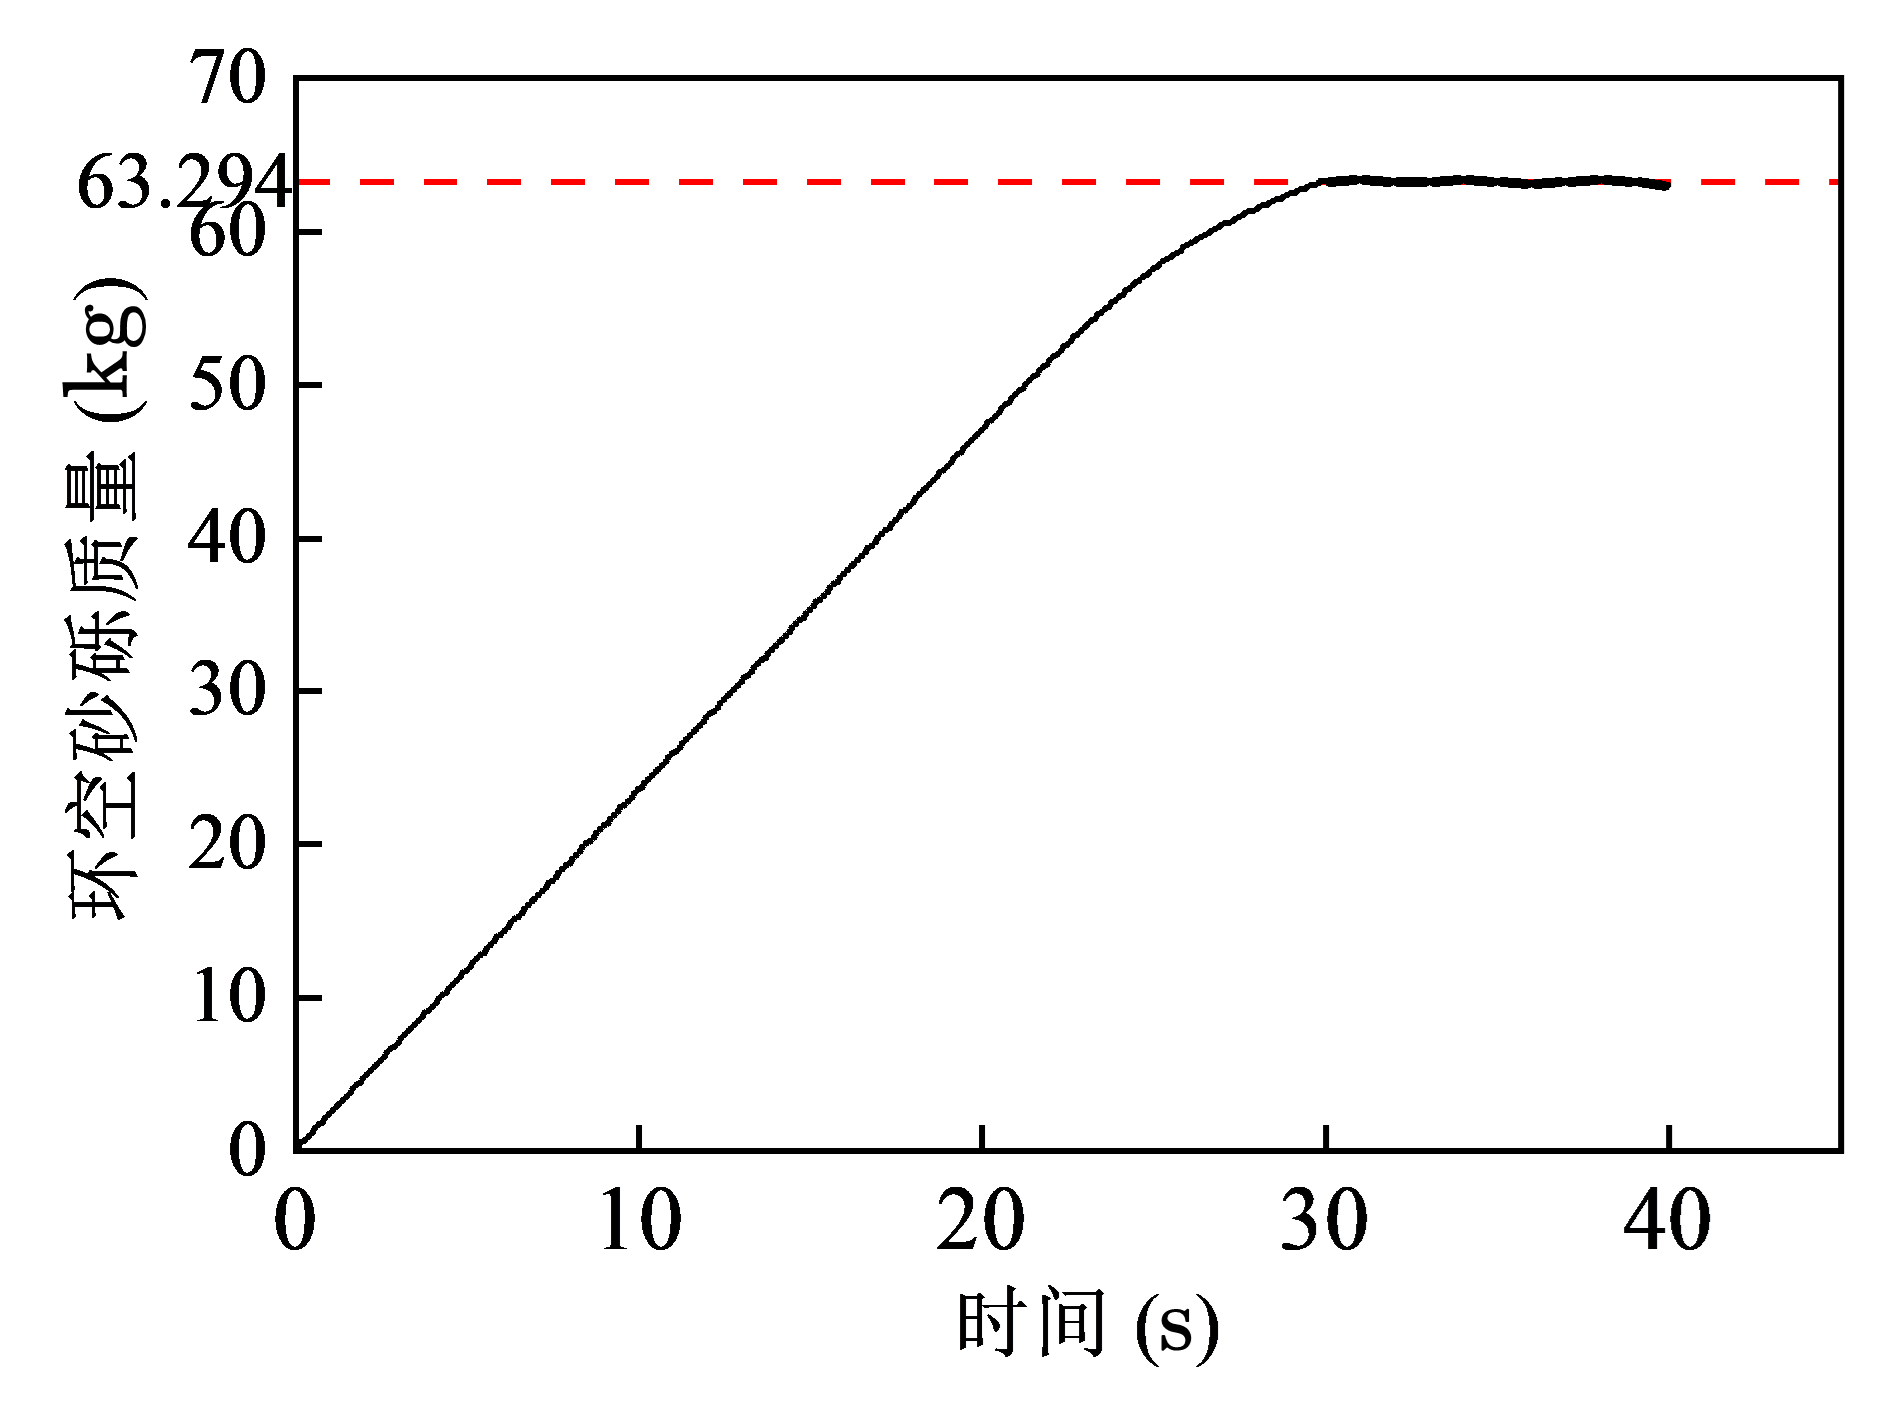
\includegraphics[width=0.5\textwidth]{figure/chapter1/sand-mass-in-annular-VS-time.png}
	\caption{环空内砂砾质量变化曲线}
	\label{fig:sand_mass_in_annular_VS_time}
\end{figure}

图\ref{fig:sand_velocity_cloud_sections}和图\ref{fig:sand_volume_fraction_cloud_sections}分别为不同位置截面砂砾轴向速度云图和砂砾体积分数云图。水平段每个截面间距 \(500\) mm，倾斜段井斜角度间隔 \(15^{\circ}\)取截面并局部放大。环空中砂砾量达到稳定后，整个环空中的砂砾分布不均匀，不同位置砂砾速度和体积分数差异大。环空上部流体流速高，下部流速趋近于零，由此可推测，在重力作用下，砂砾趋向环空下部，大部分砂砾沉降在环空下部低速区，造成砂砾难以运移，最终可能形成砂砾床。

\begin{figure}[htbp]
	\centering
	\subfloat[砂砾速度分布]{
		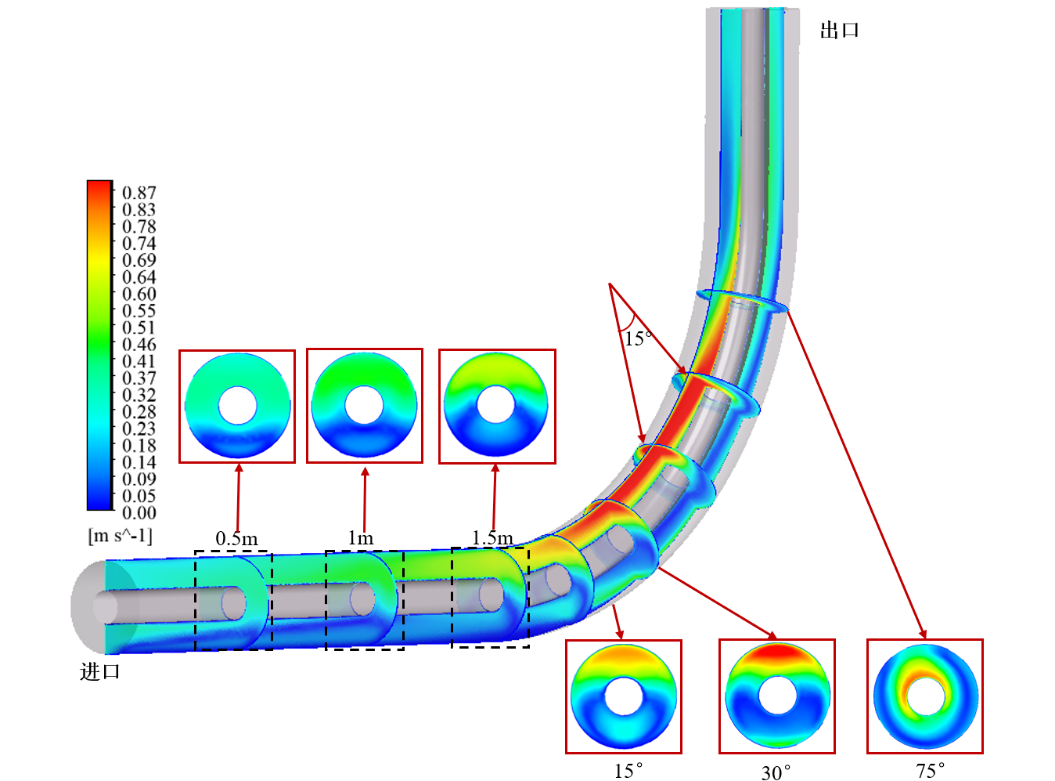
\includegraphics[width=0.6\textwidth]{figure/chapter1/sand-velocity-cloud-sections.png}
		\label{fig:sand_velocity_cloud_sections}
	}
	\hfill
	\subfloat[砂砾体积分数分布]{
	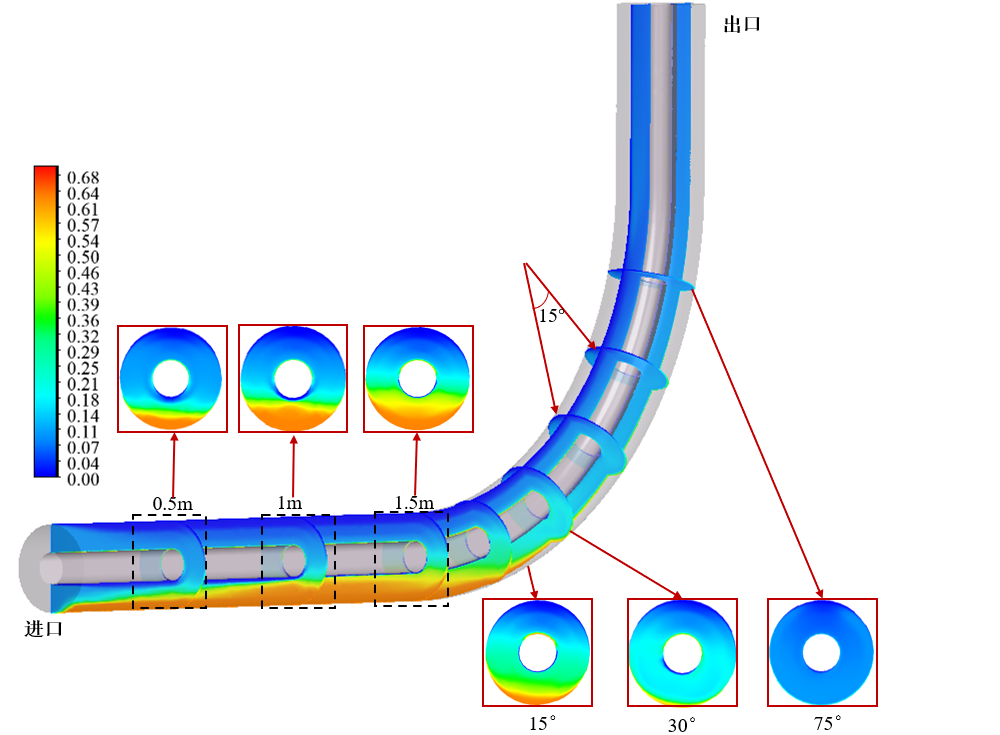
\includegraphics[width=0.6\textwidth]{figure/chapter1/sand-volume-fraction-cloud-sections.png}
	\label{fig:sand_volume_fraction_cloud_sections}
	}
	\caption{环空中砂砾轴向速度和体积分数云图（\(v_{\mathrm{in}}=0.17 \mathrm{m/s}\)）}
\end{figure}

\subsubsection{洗井液流速对环空砂砾沉积的影响}

图\ref{fig:sand_mass_in_annular_VS_time_flowrate} 为 \(v_{\mathrm{in}}=0.17,0.27,0.69 \mathrm{m/s}\)（对应泵排量分别为 25、40、100 m\(^{3}\)/h）时环空内砂砾质量随时间的变化曲线（粘度 \(\mu = 2.3 \mathrm{mPa\cdot s}\)）。由图可以看出，随着时间的延长，环空内沉降的砂砾质量趋于稳定，并且随着流速升高，环空内沉降的砂砾质量减小，达稳定的时间加快。

假设环空内体积分数最大且沉积高度最高的位置为最容易发生砂堵位置，定为砂堵点（简称 b 点）。图 \ref{fig:b_point_flowrate} 为流速 \(v_{\mathrm{in}}=0.17,0.27,0.69 \mathrm{m/s}\)三种情况下环空内砂砾的体积分数云图，随着流速的增大，砂砾体积分数逐渐减小，砂砾床高度降低，砂堵风险下降。

图\ref{fig:sand_volume_fraction_vin_dot17} 为流速为 \(v_{\mathrm{in}}=0.17\mathrm{m/s}\) 时环空内砂砾的体积分数云图，b 点出现在水平段距离入口 \(1280\) mm 处。砂砾床主要沉积在水平段，随着井斜角度增加，砂砾体积分数逐渐减小，井斜 \(\theta =75^{\circ}\) 时，砂砾体积分数接近于零，说明洗井液携砂能力较弱。\(v_{\mathrm{in}}=0.27\mathrm{m/s}\)时，b点出现在水平段距离入口 \(1150\) mm 处，砂砾床主要沉积在水平段，相对于 \(v_{\mathrm{in}}=0.17 \mathrm{m/s}\) 的工况，砂砾在井斜段体积分数有所增加，砂砾向出口运移的效率增大。当\(v_{\mathrm{in}}=0.69 \mathrm{m/s}\) 时，b 点出现在水平段距离入口 \(1530\) mm 处，直井段和小井斜段沙砾的沉积情况均较微弱。图\ref{fig:b_point_height_VS_flowrate} 为 b 点高度随洗井液流速变化曲线，随着洗井液流速增大，b 点高度呈现接近线性降低的趋势。
%既然这里提到主要沉积在水平段，可以给后面的实验佐证

\begin{figure}[htbp]
	\centering
	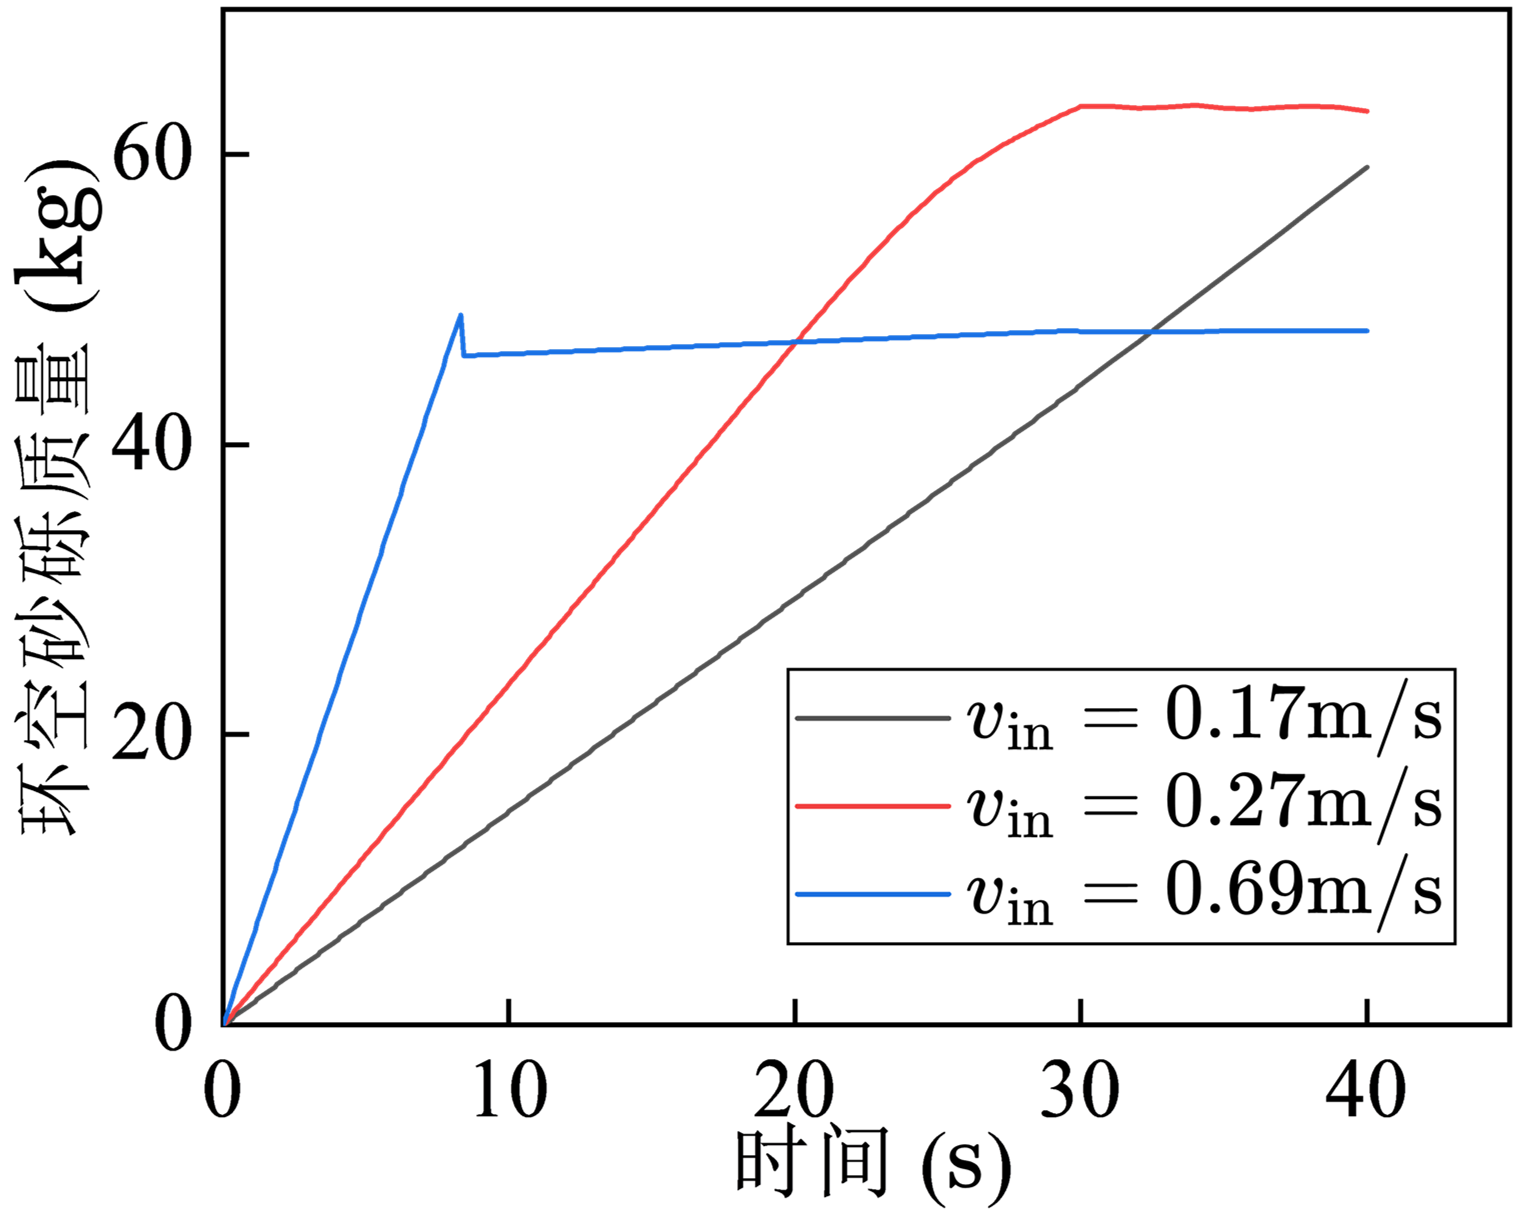
\includegraphics[width=0.5\textwidth]{figure/chapter1/sand-mass-in-annular-VS-time-flowrate.png}
	\caption{不同流速下环空内砂砾质量随时间的变化曲线\(\mu = 2.3 \mathrm{mPa\cdot s}\)}
	\label{fig:sand_mass_in_annular_VS_time_flowrate}
\end{figure}



\begin{figure}[htbp]
	\centering
	\subfloat[\(v_{\mathrm{in}}=0.17 \mathrm{m/s}\) ]{
		\includegraphics[width=0.55\textwidth]{figure/sand-volume-fraction-vin-dot17.png}
	\label{fig:sand_volume_fraction_vin_dot17}
	}
	\vspace{-1.em}
	\subfloat[\(v_{\mathrm{in}}=0.27 \mathrm{m/s}\) ]{
		\includegraphics[width=0.55\textwidth]{figure/sand-volume-fraction-vin-dot27.png}
		\label{fig:sand_volume_fraction_vin_dot27}
	}
	\vspace{-1.em}
	\subfloat[\(v_{\mathrm{in}}=0.69 \mathrm{m/s}\) ]{
		\includegraphics[width=0.55\textwidth]{figure/sand-volume-fraction-vin-dot69.png}
		\label{fig:sand_volume_fraction_vin_dot69}
	}
	\caption{流速对环空内砂砾的体积分数的影响}\label{fig:b_point_flowrate}
\end{figure}

\begin{figure}[htbp]
	\centering
	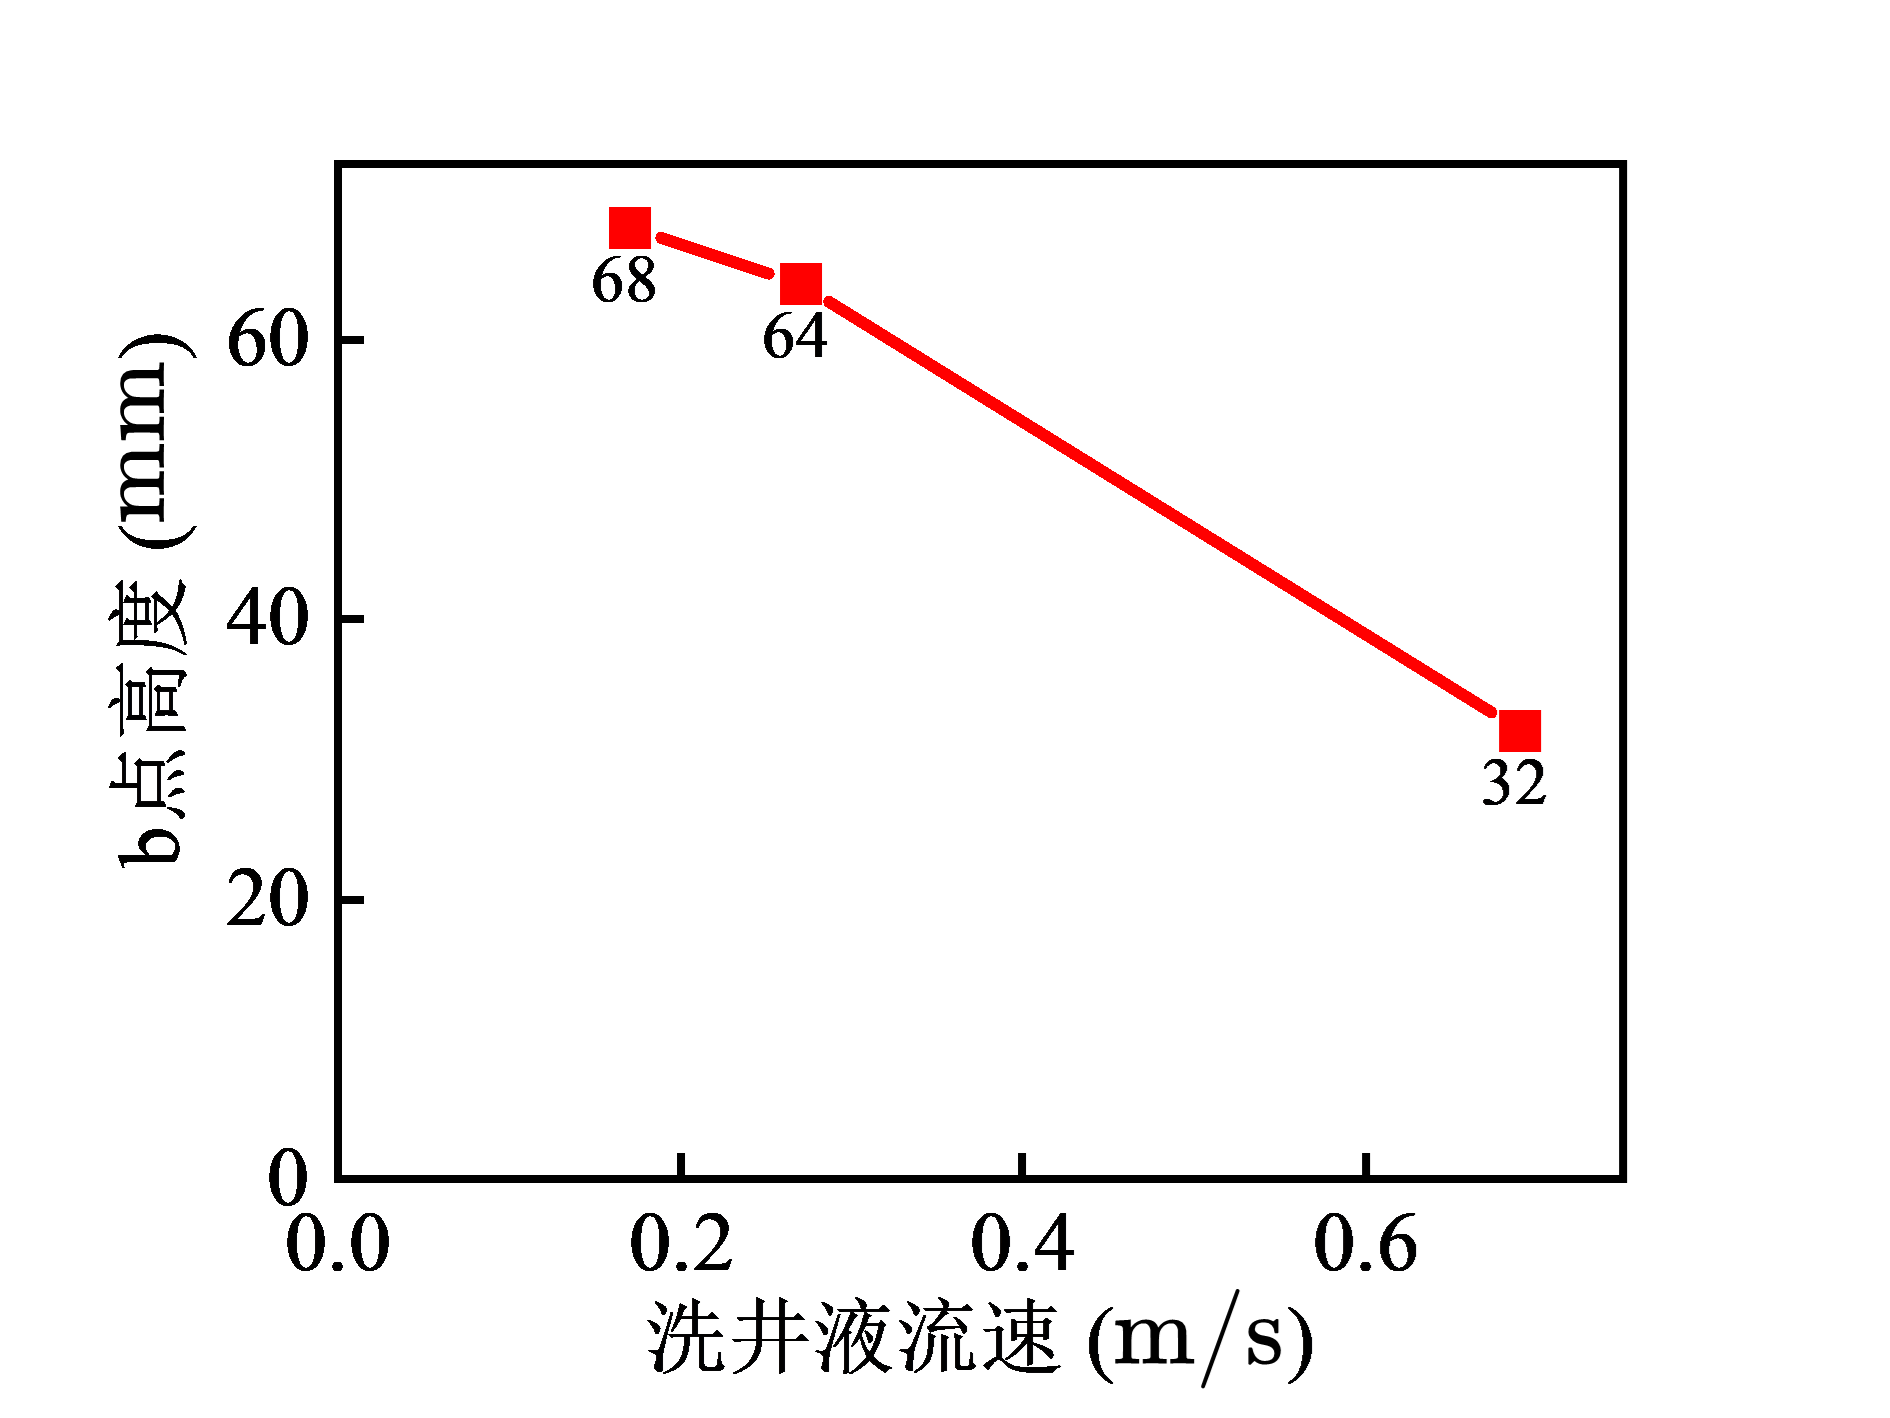
\includegraphics[width=0.6\textwidth]{figure/chapter1/b-point-height-VS-flowrate.png}
	\caption{b 点高度随洗井液流速变化曲线}
	\label{fig:b_point_height_VS_flowrate}
\end{figure}

%这个结果可以和实验进行对比

图\ref{fig:sand_volume_fraction_velocity_at_b_point_flowrate}为 b 点不同洗井液流速下砂砾体积分数和轴向速度云图。下部砂浓度高，对应沙砾的沉积区，顶部砂浓度低，砂的浓度存在明显的梯度分布。砂床的上顶面接近于平面。流速\(v_{\mathrm{in}}\)从\(0.17 \mathrm{m/s}\)增大到\(0.27 \mathrm{m/s}\)时，砂床的降低效应不显著，但增大到\(0.27 \mathrm{m/s}\)时，砂床高度明显降低。环空排量的增大，增强了流体的携砂能力，促进了砂砾颗粒在环空中的流动性，增加了砂砾颗粒能量，为砂砾运移提供了更大的拖曳力，从而有效地提高了井筒内砂砾颗粒的运移效率。因此，在实际作业中，宜尽量采用较大排量冲砂。

\begin{figure}[htbp]
	\centering
	\includegraphics[width=0.9\textwidth]{figure/sand-volume-fraction-velocity-at-b-point-flowrate.png}
	\caption{不同洗井液流速下b点所在截面砂砾体积分数和轴向速度云图}
	\label{fig:sand_volume_fraction_velocity_at_b_point_flowrate}
\end{figure}



固定 \(v_{\mathrm{in}} = 0.27\) m/s 研究洗井液粘度对环空沙砾沉积的影响。图\ref{fig:sand_mass_in_annular_VS_time_viscosity}为\(\mu =1.0\)，\(2.3\)，\(5.0 \mathrm{mPa\cdot s}\)三种粘度条件下环空内砂砾质量随时间的变化曲线。随着冲砂过程的持续，三组算例中的环空砂砾质量均逐步趋于动态平衡。洗井液粘度对砂砾沉积量及到达平衡的速率具有显著影响，随着粘度增加，颗粒受到的流体拖拽力与悬浮能力增强，显著抑制了固相颗粒在环空底部的沉降积累，使环空内最终沉降的砂砾总质量明显减小；同时，高粘度流体对颗粒运移的响应调控更为迅速，使系统达到动态平衡所需的时间显著缩短。
\begin{figure}[htbp]
	\centering
	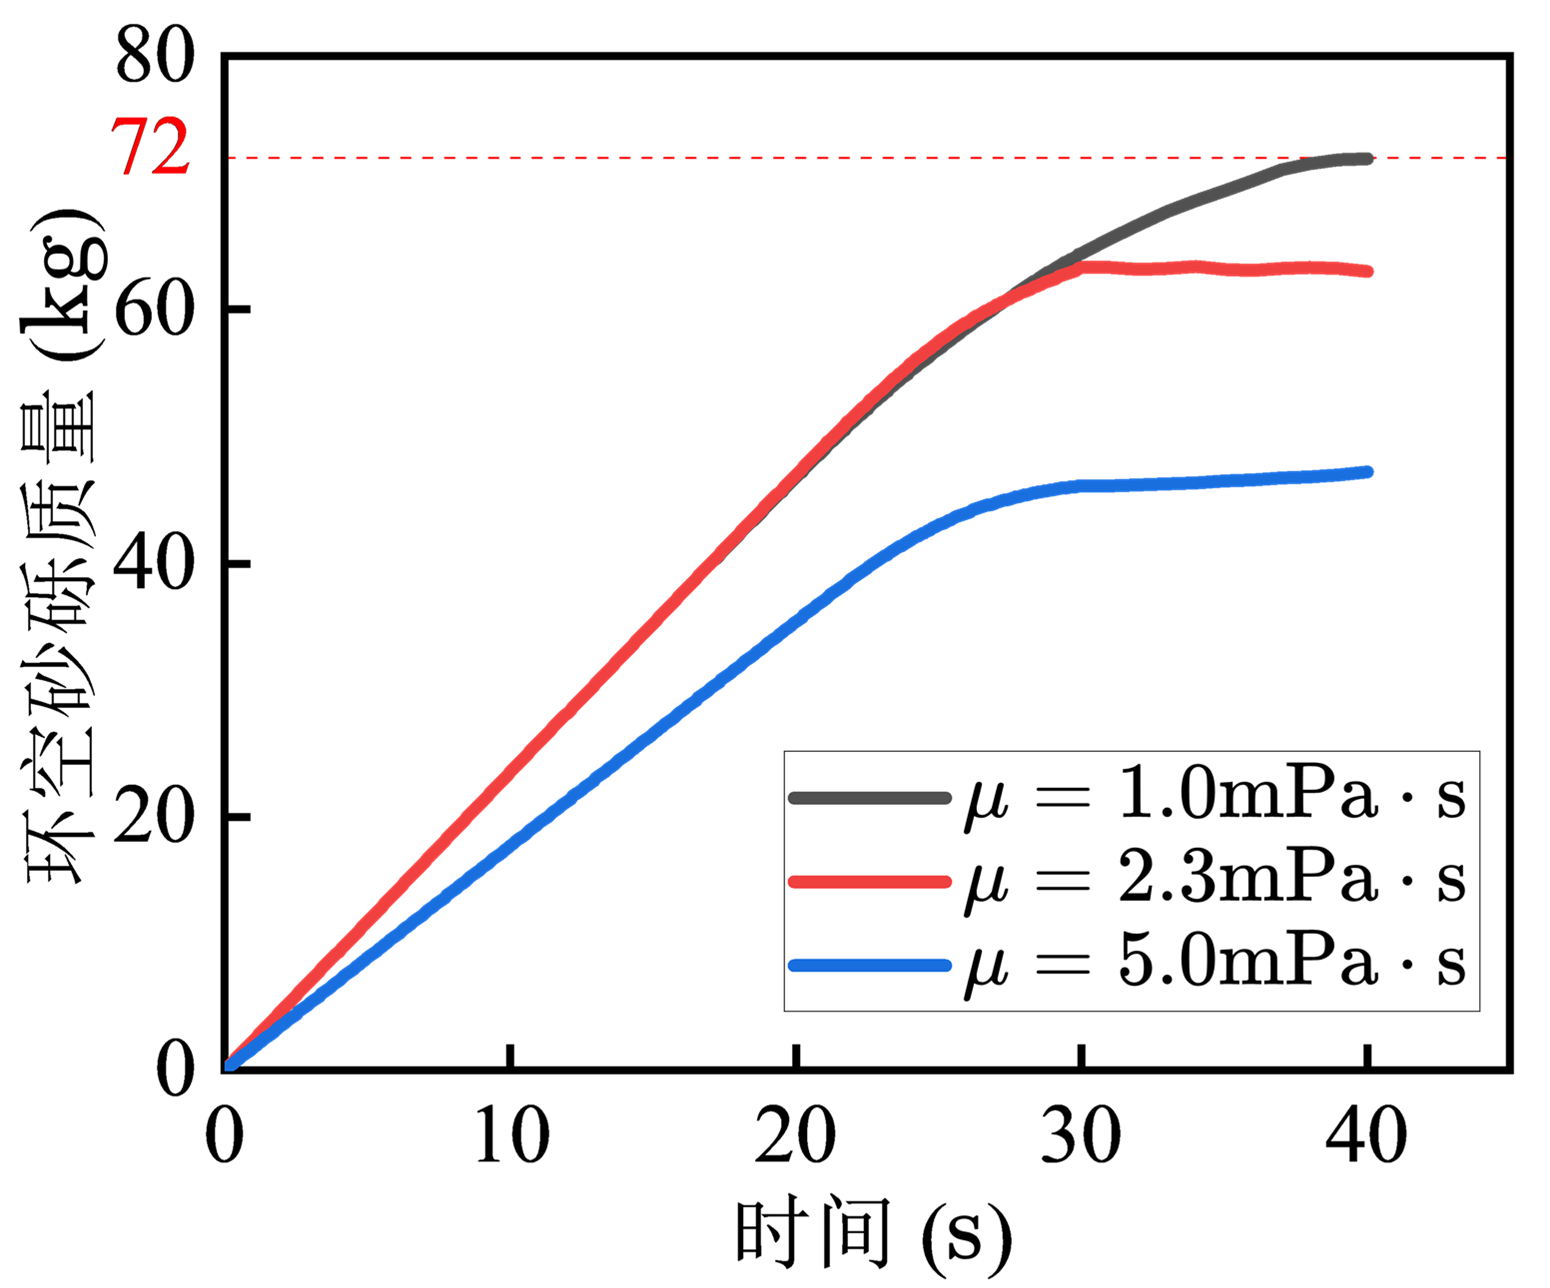
\includegraphics[width=0.5\textwidth]{figure/chapter1/sand-mass-in-annular-VS-time-viscosity.png}
	\caption{不同粘度下环空内砂砾质量随时间的变化曲线}
	\label{fig:sand_mass_in_annular_VS_time_viscosity}
\end{figure}

图\ref{fig:volume_rate_distribution_viscosity} 为 \(\mu =1.0\mathrm{mPa\cdot s}\)和\(\mu =5.0\mathrm{mPa\cdot s}\)两种情况下环空内砂砾的体积分数云图。低粘度条件（\(\mu = 1.0\ \mathrm{mPa\cdot s}\)）下，洗井液的悬浮与携砂能力较弱，砂砾主要在水平段及低倾角井斜段沉积形成明显的砂床。其中，最严重沉积点 b 点出现在水平段距离入口 \(800\text{--}1400\ \mathrm{mm}\) 区域，此时 b 点砂床高度增至 \(77.5\ \mathrm{mm}\)。随着井斜角 \(\theta\) 的增大，重力在管轴垂直方向的分量减小，砂砾沉积现象逐渐减弱；当井斜角达到 \(\theta = 75^{\circ}\) 时，环空内砂砾体积分数已接近于零。高粘度条件（\(\mu = 5.0\ \mathrm{mPa\cdot s}\)）下，流体的剪切应力与悬浮能力显著增强，有效地阻碍了砂砾向管底的沉降。此时，b 点向入口方向微移至距离入口 \(1000\ \mathrm{mm}\) 处，且砂床高度大幅削减至仅 \(25\ \mathrm{mm}\)。

图\ref{fig:b_point_height_VS_viscosity} 为 b 点砂床高度随洗井液粘度的定量变化曲线。由图可知，随着洗井液粘度的增加，b 点高度由呈现近似线性下降趋势，这一规律与提高入口流速的影响一致，表明增大洗井液粘度能够显著抑制井底及水平段的砂床积聚，有效防范井底砂堵风险。

\begin{figure}[htbp]
	\centering
	\subfloat[\(\mu =1.0 \mathrm{mPa\cdot s}\)]{
	\includegraphics[width=0.7\textwidth]{figure/sand-volume-fraction-mu-1cp.png}
	\label{fig:sand_volume_fraction_mu_1cp}
	}
	\vspace{-1em}
	\subfloat[\(\mu =5.0 \mathrm{mPa\cdot s}\)]{
	\includegraphics[width=0.7\textwidth]{figure/sand-volume-fraction-mu-5cp.png}
	\label{fig:sand_volume_fraction_mu_5cp}
	}
	\caption{不同粘度下环空内砂砾的体积分数云图}
	\label{fig:volume_rate_distribution_viscosity}
\end{figure}

\begin{figure}[htbp]
	\centering
	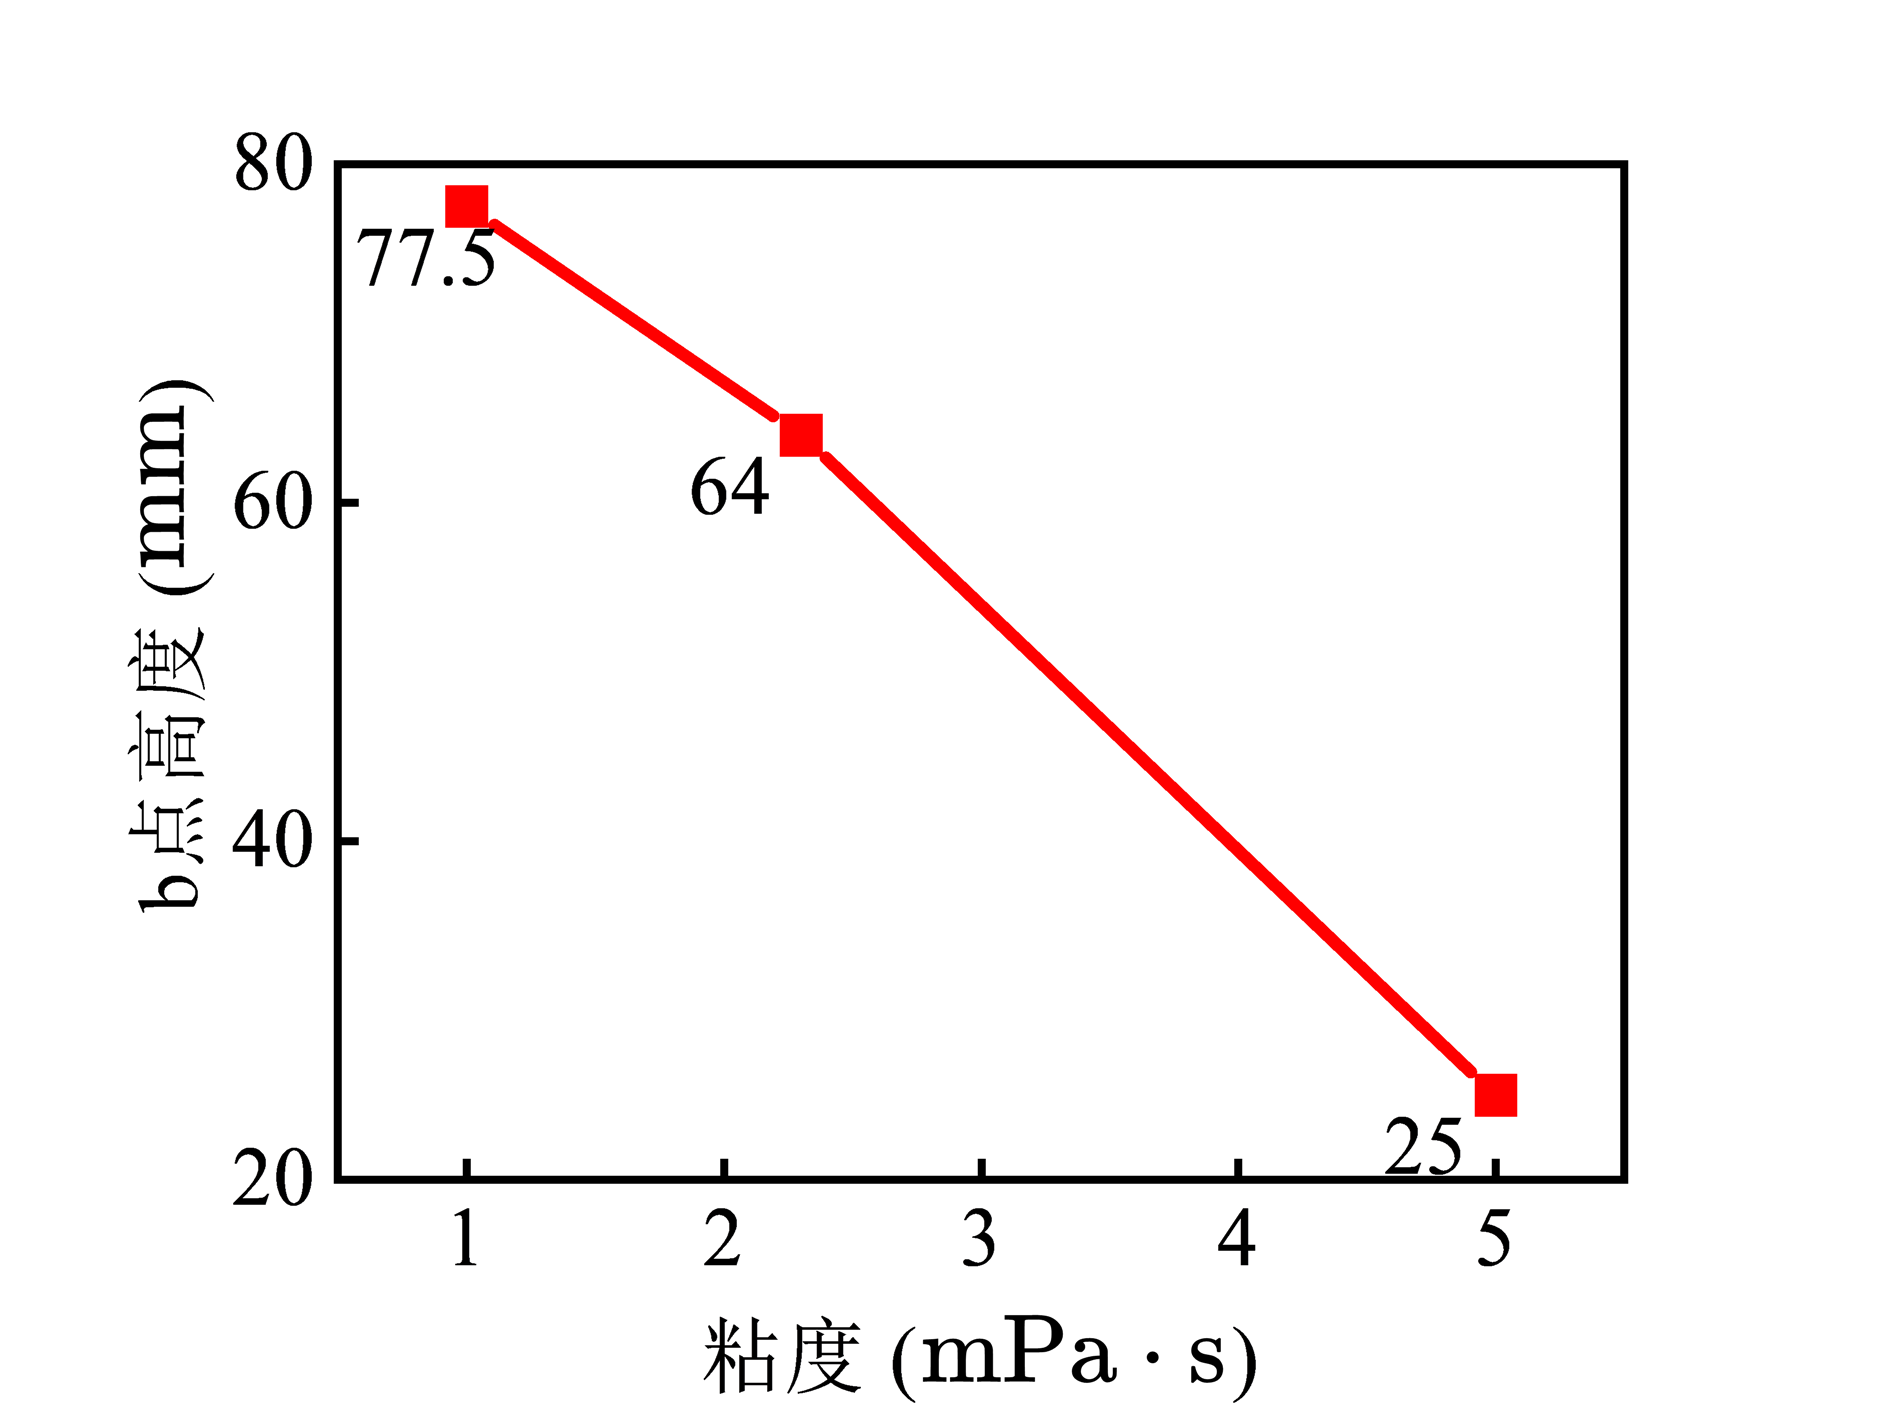
\includegraphics[width=0.5\textwidth]{figure/chapter1/b-point-height-VS-viscosity.png}
	\caption{b 点高度随洗井液粘度变化曲线}
	\label{fig:b_point_height_VS_viscosity}
\end{figure}

图\ref{fig:sand_volume_fraction_velocity_at_b_point_viscosity} 进一步展示了在相同入口流量条件下，b 点处不同粘度下的砂砾体积分数与轴向速度截面云图。低粘度（\(\mu = 1.0\ \mathrm{mPa\cdot s}\)）时，由于大量砂砾沉降在管底，形成了较厚的砂床（高体积分数红色区域占比较大），导致环空上部的有效过流截面积被严重压缩。在入口总流量恒定的前提下（\(Q = A_{\mathrm{eff}} \cdot v_{\mathrm{avg}}\)），过流面积 \(A_{\mathrm{eff}}\) 的减小逼迫上部流体以更高的局部速度挤过狭窄流道，因此出现了高达 \(1.30\ \mathrm{m/s}\) 的轴向速度峰值。随着粘度增加至 \(\mu = 5.0\ \mathrm{mPa\cdot s}\)，携砂能力增强使管底砂床高度急剧下降，环空的有效过流面积得到恢复。此时流体不再需要强行通过狭窄通道，速度分布更加均匀，使得截面最大轴向速度下降至 \(0.86\ \mathrm{m/s}\)。同时，粘度增大使得流体的剪切应力传递更为充分，速度剖面趋于平缓，增加了对砂床表面的冲刷拖拽效果，有利于固相颗粒的整体运移。

\begin{figure}[htbp]
	\centering
	\includegraphics[width=0.8\textwidth]{figure/sand-volume-fraction-velocity-at-b-point-viscosity.png}
	\caption{b 点不同洗井液粘度下砂砾体积分数和轴向速度云图}
	\label{fig:sand_volume_fraction_velocity_at_b_point_viscosity}
\end{figure}

综上所述，在实际冲砂作业中，适当增大洗井液粘度可以有效控制井底砂床高度、解除因过流面积缩小而导致的局部高流速冲蚀问题，同时防止井底卡钻与砂堵。然而，考虑到高粘度流体同时会带来更大的沿程泵压损耗，工程上应结合泵注能力合理控制洗井液粘度。考虑到砂砾在环空中的沉积以水平段为主，为了达到良好的冲砂效果，可考虑采用水力喷射工具，增加水流的脉动性，或开发过滤器等工具实现原位捞砂。
%在什么地方再提一下？实验观测那一章

\subsection{工具周围砂砾的运移及分布}

本项目涉及到的四类工具中，“四合一”工具的外部功能单元多，结构最为复杂，在工具的几何变径处会产生边界层分离和回流现象，是砂砾沉积的“危险位置”。于是，本文选择“四合一”工具的扶正器和强磁位置作为对象，研究砂砾在此处的沉积行为。建立强磁部位与 7\inch 井筒环空流体仿真模型。根据表\ref{tab:real_sand_parameter}建立相对应的大小与数量的砂砾颗粒仿真模型（具体参数见表\ref{tab:simulation_sand_parameter}）。仿真模型数据见表 \ref{tab:simulation_parameter_4in1}。在 EDEM 软件中，颗粒产生于“颗粒工厂”，其初始速度、角速度为零，角度随机。研究不同环空流速下（\(v_{\mathrm{c}}=0.37\) m/s、\(0.59\) m/s）砂砾的运移及沉降规律，探究砂砾是否会出现沉积或者堵塞现象。计算结果如图 \ref{fig:sand_distribution_annular_vin} 所示。

\begin{table}[H]
	\centering
	\caption{“四合一”工具砂砾沉积仿真模型数据}
	\label{tab:simulation_parameter_4in1}
	\begin{tabularx}{.9\textwidth}{CCCC}
		\toprule
		名称 & 符号 & 数值 & 单位 \\
		\midrule
		水平井筒长度 & \(L\) & 1.5 & m \\
		井筒直径 & \(D_{\mathrm{H}}\) & 177.8 & mm \\
		钻杆直径 & \(D_{\mathrm{P}}\) & 88.9 & mm \\
		颗粒密度 & \(\rho_{\mathrm{P}}\) & 2650.0 & kg/m\(^{3}\) \\
		洗井液密度 & \(\rho_{\mathrm{l}}\) & 1000.0 & kg/m\(^{3}\) \\
		井斜角 & \(\theta\) & 90.0 & \(^{\circ}\) \\
		洗井液入口流速 & \(v_{\mathrm{c}}\) & 0.37、0.59 & m/s \\
		洗井液粘度 & \(\mu\) & 1.0 & mPa·s \\
		\bottomrule
	\end{tabularx}
\end{table}

\begin{table}[H]
	\centering
	\caption{仿真颗粒粒径及数量分布}
	\label{tab:simulation_sand_parameter}
	\begin{tabularx}{.9\textwidth}{CCCC}
		\toprule
		类型 & 砂砾颗粒数量/个 & 粒径分布比例/\% & 粒径大小/\(\mu\)m \\
		\midrule
		粗砂 & $1000$ & $1.0$ & $750$ \\
		中砂 & $35000$ & $35.0$ & $375$ \\
		细砂 & $47000$ & $47.0$ & $187.5$ \\
		极细砂 & $14000$ & $14.0$ & $93.75$ \\
		粗粉砂 & $2000$ & $3.0$ & $46.875$ \\
		\bottomrule
	\end{tabularx}
\end{table}

\begin{figure}[htbp]
	\centering
	\includegraphics[width=\textwidth]{figure/tool-and-wellbore-simulation-model.png}
	\caption{工具及井筒仿真模型}
	\label{fig:tool_wellbore_model}
\end{figure}

图 1.9 描述的是洗井液流速 \(0.37\) m/s 下井筒与工具环空内砂砾颗粒分布情况。从图可以看出，部分砂砾颗粒由于重力作用会在工具前端产生堆积，同时砂砾颗粒会随着工具的导流结构进行运移，在强磁部件的凹槽内也会有少量的砂砾堆积现象。

% \begin{figure}[htbp]
% 	\centering
% 	\includegraphics[width=\textwidth]{figure/sand-distribution-tool-vin-dot37.png}
% 	\caption{洗井液流速 0.37 m/s 下井筒与工具环空内砂砾颗粒分布}
% 	\label{fig:sand_distribution_tool_vin_dot37}
% \end{figure}

图 1.10 描述的是相同时间步环空流速 \(0.37\) m/s、\(0.59\) m/s 下砂砾颗粒分布。从图中可以看出，环空流速增大时，靠近压力出口的砂砾颗粒越多，砂砾颗粒的运移效率明显加快。在相同时间步下，环空流速越大，颗粒运移速度越快。由于环空流速增大，流体的拖曳力增大，砂砾颗粒在轴向的速度增大，砂砾颗粒由于重力作用产生的沉积位置与流体入口的距离也变远。

\begin{figure}[htbp]
	\centering
	\subfloat[$v_\mathrm{c}=0.37 \mathrm{m/s}$]{%
		\includegraphics[width=0.98\textwidth]{figure/sand-distribution-annular-vin-dot37.png}
		\label{fig:sand_distribution_annular_vin_dot37}
	}
	\vspace{0pt}
	\subfloat[$v_\mathrm{c}=0.59 \mathrm{m/s}$]{%
		\includegraphics[width=0.98\textwidth]{figure/sand-distribution-annular-vin-dot59.png}
		\label{fig:sand_distribution_annular_vin_dot59}
	}
	\caption{相同时间步不同环空流速下砂砾颗粒分布}
	\label{fig:sand_distribution_annular_vin}
\end{figure}

通过仿真发现，在冲砂作业时，如果环空流体中砂砾体积分数越大，越容易在工具与井筒下壁之间的环空中产生沉积，环空流速增大，砂砾运移效率加快，建议在作业时增大洗井液流速即增大冲砂液排量以减小砂砾堆积的风险，降低砂堵概率。同时，工具的导流结构也对砂砾运移起到关键作用，砂砾颗粒会随着工具的导流结构进行运移，降低了砂堵的风险，为工具安全作业提供保障。

上述研究仅仅从宏观上观测砂砾在井筒环空中的运移情况，无法提取井筒环空中不同具体位置的砂砾体积分数、砂砾速度及砂砾床厚度等数据。为此，本研究考虑井筒环空不同位置的砂砾量，基于欧拉液固两相流模型和 SST \( k\)-\(\omega\) 模型，建立了三维井眼环空颗粒运移模型，在分析砂砾体积分数和砂砾速度的基础上，通过 Fluent 分析整个环空中砂砾质量，提出了环空内含有颗粒质量的变化方法，分析了环空流速、井斜角度、洗井液粘度等对环空内沉降的砂床高度的影响。所得结论对水平井和大位移井环空内井筒清洁和高效作业具有指导意义。

%以下是水平井筒内砂砾运移及分布规律研究的具体内容，由于模拟结果目前和实验对不上，所以，先不展示。

% 为了模拟井筒内携带颗粒的特性，模型需要通过设计一个环形空间来实现。研究中建立了内径 \(\phi 88.9\) mm、外径 \(\phi 244.475\) mm、\(\phi 177.8\) mm、总长度为 \(1.5\) m 的光滑管柱，用于模拟钻杆（\(3\)-\(1/2'\)）和井筒（\(9\)-\(5/8'\)、\(7'\)），套管和钻杆同心。在模拟过程中，内部钻杆固定，钻井液以一定速度垂直于入口方向流入环形空间，并从另一端出口流出。环空模型如图 1.5、图 1.6 所示。计算采用了非稳态 \(k-\varepsilon\) 湍流模型，将颗粒设置为离散相，并利用多面体网格进行建模。边界条件包括速度入口、压力出口，管壁采用无滑移条件。一般计算参数具体数值见表 1.1，重力方向始终竖直向下，对于不同 \(\theta\) 的情况，流体域旋转相应角度。

% \begin{figure}[htbp]
% 	\centering
% 	\includegraphics[width=0.9\textwidth]{figure/fluid-domain-geometry.png}
% 	\caption{流体域几何模型示意图}
% 	\label{fig:fluid_domain_geometry}
% \end{figure}

% \begin{figure}[htbp]
% 	\centering
% 	\includegraphics[width=0.9\textwidth]{figure/fluid-domain-polyhedral-mesh.jpg}
% 	\caption{流体域多面体单元离散示意图}
% 	\label{fig:fluid_domain_mesh}
% \end{figure}
